\documentclass[12pt]{article}

%Paquetes
\usepackage{titlesec}
\usepackage[dvipsnames]{xcolor}
\usepackage{lipsum}
\usepackage{fontspec}
\usepackage{graphicx} %Imágenes
\usepackage{colortbl}
\usepackage{setspace}
\usepackage[a4paper]{geometry}
\usepackage{fancyhdr}
\usepackage[babel]{csquotes}
\usepackage[spanish, english]{babel}
\usepackage{apacite} % Norma APA bibliografía
\usepackage{natbib} %Bibliografía
\usepackage[nottoc]{tocbibind}
\usepackage[acronym,nonumberlist,toc]{glossaries} % Configuraciones glosario
\usepackage{glossary-superragged} %Configuraciones glosario
\usepackage[hang,flushmargin]{footmisc}
\usepackage{etoolbox}
\usepackage[hidelinks, breaklinks=true]{hyperref}
\usepackage{booktabs} % Tablas
\usepackage{tabularx}
\usepackage{float}
\usepackage{hyperref}
\usepackage{nameref}
\usepackage{verbatim} % Para comentarios multilinea
\usepackage{longtable} % tablas grandes
\usepackage{listings}
\usepackage{color}
\usepackage{fontawesome5} % Iconos de FontAwesome
\usepackage{caption}
\usepackage{subcaption}
\usepackage{tikz} % diagramas
\usetikzlibrary{arrows.meta, positioning}
\usepackage{rotating} % para rotar tablas
\usepackage{makecell}
\usepackage{pdflscape} % rotar páginas
\usepackage{amsmath}
\usepackage{amsfonts}

\definecolor{myred}{HTML}{E74C3C}
\definecolor{mygreen}{HTML}{27AE60}

\definecolor{dkgreen}{RGB}{0,0.6,0}
\definecolor{gray}{RGB}{0.5,0.5,0.5}
\definecolor{mauve}{RGB}{0.58,0,0.82}
\definecolor{delim}{RGB}{20,105,176}
\definecolor{numb}{RGB}{106, 109, 32}
\definecolor{string}{RGB}{0.64,0.08,0.08}

%%%%%%%%%%%%%%%%%%%%%%%%%%%%%%%%%%%%%%%%%%%%%%%%%%%%%%
%%%%%%%%%%% YAML syntax highlighting %%%%%%%%%%%%%%%%%

% http://tex.stackexchange.com/questions/152829/how-can-i-highlight-yaml-code-in-a-pretty-way-with-listings

% here is a macro expanding to the name of the language
% (handy if you decide to change it further down the road)
\newcommand\YAMLcolonstyle{\color{red}\mdseries}
\newcommand\YAMLkeystyle{\color{black}\bfseries}
\newcommand\YAMLvaluestyle{\color{blue}\mdseries}

\makeatletter

\newcommand\language@yaml{yaml}

\expandafter\expandafter\expandafter\lstdefinelanguage
\expandafter{\language@yaml}
{
	keywords={true,false,null,y,n},
	keywordstyle=\color{darkgray}\bfseries,
	basicstyle=\YAMLkeystyle,                                 % assuming a key comes first
	sensitive=false,
	comment=[l]{\#},
	morecomment=[s]{/*}{*/},
	commentstyle=\color{purple}\ttfamily,
	stringstyle=\YAMLvaluestyle\ttfamily,
	moredelim=[l][\color{orange}]{\&},
	moredelim=[l][\color{magenta}]{*},
	moredelim=**[il][\YAMLcolonstyle{:}\YAMLvaluestyle]{:},   % switch to value style at :
	morestring=[b]',
	morestring=[b]",
	literate =    {---}{{\ProcessThreeDashes}}3
	{>}{{\textcolor{red}\textgreater}}1     
	{|}{{\textcolor{red}\textbar}}1 
	{\ -\ }{{\mdseries\ -\ }}3,
}

% switch to key style at EOL
\lst@AddToHook{EveryLine}{\ifx\lst@language\language@yaml\YAMLkeystyle\fi}
\makeatother

\newcommand\ProcessThreeDashes{\llap{\color{cyan}\mdseries-{-}-}}

%%%%%%%%%%% YAML syntax highlighting %%%%%%%%%%%%%%%%%
%%%%%%%%%%%%%%%%%%%%%%%%%%%%%%%%%%%%%%%%%%%%%%%%%%%%%%

% Python language definition
\lstset{frame=tb,
	language=Python,
	aboveskip=3mm,
	belowskip=3mm,
	showstringspaces=false,
	columns=flexible,
	basicstyle={\small\ttfamily},
	numbers=none,
	numberstyle=\tiny\color{gray},
	keywordstyle=\color{blue},
	commentstyle=\color{dkgreen},
	stringstyle=\color{mauve},
	breaklines=true,
	breakatwhitespace=true,
	tabsize=3
}

% Kotlin language definition
\lstdefinelanguage{Kotlin}{
	comment=[l]{//},
	commentstyle={\color{gray}\ttfamily},
	emph={filter, first, firstOrNull, forEach, lazy, map, mapNotNull, println},
	emphstyle={\color{OrangeRed}},
	identifierstyle=\color{black},
	keywords={!in, !is, abstract, actual, annotation, as, as?, break, by, catch, class, companion, const, constructor, continue, crossinline, data, delegate, do, dynamic, else, enum, expect, external, false, field, file, final, finally, for, fun, get, if, import, in, infix, init, inline, inner, interface, internal, is, lateinit, noinline, null, object, open, operator, out, override, package, param, private, property, protected, public, receiver, reified, return, return@, sealed, set, setparam, super, suspend, tailrec, this, throw, true, try, typealias, typeof, val, var, vararg, when, where, while},
	keywordstyle={\color{NavyBlue}\bfseries},
	escapeinside={//(`}{`)},
	morecomment=[s]{/*}{*/},
	morestring=[b]",
	morestring=[s]{"""*}{*"""},
	ndkeywords={@Composable, @Preview, @Deprecated, @JvmField, @JvmName, @JvmOverloads, @JvmStatic, @JvmSynthetic, Array, Byte, Double, Float, Int, Integer, Iterable, Long, Runnable, Short, String, Any, Unit, Nothing},
	ndkeywordstyle={\color{BurntOrange}\bfseries},
	sensitive=true,
	stringstyle={\color{ForestGreen}\ttfamily},
}

% JSON definition

\lstdefinelanguage{json}{
	numbers=left,
	numberstyle=\small,
	frame=single,
	rulecolor=\color{black},
	showspaces=false,
	showtabs=false,
	breaklines=true,
	postbreak=\raisebox{0ex}[0ex][0ex]{\ensuremath{\color{gray}\hookrightarrow\space}},
	breakatwhitespace=true,
	basicstyle=\ttfamily\small,
	upquote=true,
	morestring=[b]",
	stringstyle=\color{string},
	literate=
	*{0}{{{\color{numb}0}}}{1}
	{1}{{{\color{numb}1}}}{1}
	{2}{{{\color{numb}2}}}{1}
	{3}{{{\color{numb}3}}}{1}
	{4}{{{\color{numb}4}}}{1}
	{5}{{{\color{numb}5}}}{1}
	{6}{{{\color{numb}6}}}{1}
	{7}{{{\color{numb}7}}}{1}
	{8}{{{\color{numb}8}}}{1}
	{9}{{{\color{numb}9}}}{1}
	{\{}{{{\color{delim}{\{}}}}{1}
	{\}}{{{\color{delim}{\}}}}}{1}
	{[}{{{\color{delim}{[}}}}{1}
	{]}{{{\color{delim}{]}}}}{1},
}

%Variables
\definecolor{gray80}{gray}{.80}
\definecolor{blueUnir}{HTML}{0098CD}

\geometry{top=2.5cm, bottom=2.5cm, left=3.0cm, right=2.0cm}
\setmainfont{Calibri}
\spacing{1.5} %Interlineado fijo
\setlength{\parskip}{6pt} %6 puntos de espaciado entre párrafos
\setlength{\parindent}{0cm} %Eliminar sangría
\setlength{\footnotesep}{0pt} %Espaciado entre notas
\setlength{\skip\footins}{1.5cm} %Espaciado entre raya y texto
\renewcommand{\footnotelayout}{\small\baselineskip=10pt} % Interlineado sencillo

\fancyhf{}
\pagestyle{fancy}
\rhead[\fontsize{10pt}{12pt}\setmainfont{Calibri Light}\selectfont Jon Inazio Sánchez Martínez\\Predicción de tráfico mediante aprendizaje profundo y Transformers]{\fontsize{10pt}{12pt}\setmainfont{Calibri Light}\selectfont Jon Inazio Sánchez Martínez\\Predicción de tráfico mediante aprendizaje profundo y Transformers} 
\renewcommand{\headrulewidth}{0pt}
%\renewcommand{\footrulewidth}{1pt}
\rfoot[]{\thepage}
\setcounter{tocdepth}{3} 
\setcounter{secnumdepth}{5}
\newcommand\fh{\babelhyphen{hard}}

\titleformat*{\section}{\fontsize{18pt}{18}\selectfont\color{blueUnir}\setmainfont{Calibri Light}} 
\titleformat*{\subsection}{\fontsize{14pt}{14}\selectfont\color{blueUnir}\setmainfont{Calibri Light}} 
\titleformat*{\subsubsection}{\fontsize{12pt}{12}\selectfont\setmainfont{Calibri}\bfseries}

%
% Acrónimos
%
% La forma de definir un acrónimo es la siguiente:
% \newacronym{id}{siglas}{descripción}
% Donde:
% 	'id' es como vas a llamarlo desde el documento.
%	'siglas' son las siglas del acrónimo.
%	'descripción' es el texto que representan las siglas.
%
% Para usarlo en el documento tienes 4 formas:
% \gls{id} - Añade el acrónimo en su forma larga y con las siglas si es la primera vez que se utiliza, el resto de veces solo añade las siglas. (No utilices este en títulos de capítulos o secciones).
% \glsentryshort{id} - Añade solo las siglas de la id
% \glsentrylong{id} - Añade solo la descripción de la id
% \glsentryfull{id} - Añade tanto  la descripción como las siglas

\newacronym{dl}{DL}{Deep Learning o Aprendizaje Profundo}
\newacronym{its}{ITS}{Sistemas Inteligentes de Transporte}
\newacronym{capv}{CAPV}{Comunidad Autónoma del País Vasco}
\newacronym{rnn}{RNN}{Recurrent Neural Networks o Redes Neuronales Recurrentes}
\newacronym{cnn}{CNN}{Convolutional Neural Networks o Redes Neuronales Convolucionales}
\newacronym{lstm}{LSTM}{Long Short-Term Memory}
\newacronym{gnn}{GNN}{Graph Neural Networks}
\newacronym{gru}{GRU}{Gated Recurrent Units}
\newacronym{gcn}{GCN}{Graph Convolutional Networks}
\newacronym{ggnn}{GGNN}{Gated Graph Neural Networks}
\newacronym{gat}{GAT}{Graph Attention Networks}
\newacronym{mlp}{MLP}{Multi Layer Perceptron o Perceptrones Multi Capa}
\newacronym{rmse}{RMSE}{Root Mean Square Error o Error Cuadrático Medio}
\newacronym{mape}{MAPE}{Mean Absolute Percentage Error o Error Porcentual Absoluto Medio}
\newacronym{mae}{MAE}{Mean Absolute Error o Error Medio Absoluto}
\newacronym{mre}{MRE}{Mean Relative Error o Error Medio Relativo}
\newacronym{svr}{SVR}{Support Vector Regression}
\newacronym{svm}{SVM}{Support Vector Machines}
\newacronym{rf}{RF}{Random Forests}
\newacronym{knn}{KNN}{K-Nearest Neighbors}
\newacronym{arima}{ARIMA}{AutoRegressive Integrated Moving Average}
\newacronym{sarima}{SARIMA}{Seasonal AutoRegressive Integrated Moving Average}
\newacronym{gpu}{GPU}{Graphics Processing Unit}
\newacronym{ram}{RAM}{Random Access Memory}
\newacronym{ssd}{SSD}{Solid State Drive}

%
% Glosario
%
%\newglossaryentry{latex}
%{
	%	name=latex,
	%	description={Is a mark up language specially suited for scientific documents}
	%}
\newglossaryentry{api}{
	name=API,
	description={Interfaz de programación de aplicaciones. Conjunto de funciones y definiciones que permiten la comunicación entre sistemas de software}
}

\newglossaryentry{json}{
	name=JSON,
	description={JavaScript Object Notation. Formato ligero y estructurado de intercambio de datos, ampliamente utilizado en APIs y configuraciones}
}

\newglossaryentry{geojson}{
	name=GeoJSON,
	description={Extensión del formato JSON para representar objetos geoespaciales como puntos, líneas, polígonos o colecciones de geometrías}
}

\newglossaryentry{uml}{
	name=UML,
	description={Unified Modeling Language. Lenguaje de modelado visual estandarizado para representar sistemas software desde distintas perspectivas (estructural, de comportamiento, etc.)}
}

\newglossaryentry{nosql}{
	name=NoSQL,
	description={Modelo de bases de datos no relacional orientado a documentos, grafos, columnas o pares clave-valor, ideal para sistemas distribuidos, escalables y flexibles}
}

\newglossaryentry{arquitectura-hexagonal}{
	name=arquitectura hexagonal,
	description={Estilo de diseño de software que promueve la separación de la lógica del dominio respecto a la infraestructura, facilitando el mantenimiento, las pruebas y la escalabilidad}
}

\newglossaryentry{aforo}{
	name=aforo,
	description={Medida del flujo de vehículos que pasan por un punto determinado de una carretera o vía en un periodo de tiempo concreto. Utilizado para analizar la intensidad y distribución del tráfico.}
}

\newglossaryentry{redviaria}{
	name=red viaria,
	description={Conjunto de infraestructuras y vías (carreteras, autopistas, calles) que conforman la red de transporte terrestre de una región o país.}
}

\newglossaryentry{aforador}{
	name=aforador,
	description={Dispositivo utilizado para medir el número de vehículos que pasan por un punto de la red viaria, registrando el flujo de tráfico}
}

\newglossaryentry{resampling}{
	name=resampling,
	description={Proceso de agregación o interpolación de datos temporales para ajustarse a una nueva frecuencia}
}

\newglossaryentry{ventana}{
	name=ventana deslizante,
	description={Técnica que permite recorrer una serie temporal generando subconjuntos de datos consecutivos}
}

\newglossaryentry{normalizacion}{
	name=normalización,
	description={Transformación de los datos para que tengan media cero y desviación estándar uno u otro rango definido}
}

\newglossaryentry{onnx}{
	name=ONNX,
	description={Open Neural Network Exchange. Formato abierto y estandarizado para representar modelos de aprendizaje automático, diseñado para facilitar la interoperabilidad entre diferentes frameworks de deep learning como PyTorch, TensorFlow, Keras o Scikit-learn}
}


\newglossaryentry{design_pattern:builder}{
	name=Builder,
	description={Separa la construcción de un objeto complejo de su representación, permitiendo que el mismo proceso de construcción pueda crear diferentes representaciones. Utilizado en la generación del dataset a través de la clase \texttt{MobilitySnapshotBuilder}}
}
\newglossaryentry{design_pattern:repository}{
	name=Repository,
	description={Media entre el dominio y las capas de mapeo de datos, proporcionando una interfaz similar a una colección para acceder a los objetos del dominio. Todas las operaciones de acceso a datos (\texttt{FlowRepository}, \texttt{MeterRepository}, etc.) se abstraen en repositorios desacoplados}
}
\newglossaryentry{design_pattern:servicelayer}{
	name=Service Layer,
	description={Define los límites de una aplicación y las operaciones disponibles, coordinando la respuesta de la aplicación en cada operación. La lógica de negocio reside en servicios como \texttt{FlowService}, \texttt{MeterService}, \texttt{IncidenceService}}
}
\newglossaryentry{design_pattern:dto}{
	name=Data Transfer Object,
	description={Es un objeto que transporta datos entre procesos, generalmente para reducir el número de llamadas a métodos remotos. Se emplean DTOs para el intercambio de datos entre capas, evitando el acoplamiento con los modelos de persistencia.}
}
\newglossaryentry{design_pattern:helper_utility}{
	name=Helper/Utility,
	description={Helper: Proporciona funcionalidad reutilizable y de bajo nivel a otras clases, a menudo a través de métodos estáticos, para evitar la duplicación de código. Utility: Es una clase que agrupa métodos estáticos con funcionalidades comunes y reutilizables que no dependen del estado de ningún objeto. Utilidades para parseo, validación y transformación de datos (por ejemplo, para el tratamiento de ficheros XML meteorológicos)}
}
\newglossaryentry{design_pattern:facade}{
	name=Facade,
	description={Ofrece una interfaz unificada y simplificada a un conjunto de interfaces en un subsistema más complejo, facilitando su uso. Fachadas que agrupan operaciones complejas en interfaces sencillas, facilitando la integración con servicios externos.}
}
\newglossaryentry{design_pattern:factory_singleton}{
	name=Factory/Singleton,
	description={Factory: Se encarga de crear objetos sin especificar la clase exacta del objeto que se creará, delegando esta lógica a una subclase. Garantiza que una clase tenga una única instancia y proporciona un punto de acceso global a ella. Empleados para instanciar objetos según el origen de datos y para servicios centrales, respectivamente.}
}
\makeglossaries

\makeatletter
\patchcmd{\@footnotetext}{\footnotesize}{\fontsize{10pt}{12pt}\setmainfont{Calibri}}{}{}
\makeatother

\addto\captionsspanish{%
	\renewcommand*\contentsname{Índice de contenidos}
	\renewcommand{\listtablename}{Índice de tablas} 
	\renewcommand{\tablename}{Tabla} 
	%\renewcommand{\bibname}{Referencia bibliográfica}
}

\titlespacing*{\paragraph}{0pt}{9pt}{0.5ex}
\titleformat{\paragraph}[block]{\normalsize}{\theparagraph}{.5em}{\mdseries}
\titlespacing*{\subparagraph}{0pt}{9pt}{0.5ex}
\titleformat{\subparagraph}[block]{\normalsize}{\thesubparagraph}{.5em}{\mdseries}

\renewenvironment{description}
{\list{}{\labelwidth0pt\itemindent-\leftmargin\parsep0pt\itemsep0pt\let\makelabel\descriptionlabel}}{\endlist}

\selectlanguage{spanish}
\begin{document}
	
	\begin{titlepage}
	
	% Quitar dependiendo si título es igual que los demás
	%\newgeometry{top=2.5cm, bottom=2.5cm, left=2.0cm, right=2.0cm}
	
	\centering
	\vspace{3cm}
	
\includegraphics[width=0.60\textwidth]{includes/logoUnir.eps}\\	
	{\Huge Universidad Internacional de La Rioja \\}
	{\LARGE Escuela Superior de Ingeniería y Tecnología \\}
	\vspace{3cm}
	\setmainfont{Calibri Light}
	{\Large Máster Universitario en Inteligencia Artificial\\}
	\setmainfont{Calibri}
	{\Huge\textcolor{blueUnir}{Predicción de tráfico mediante aprendizaje profundo y Transformers} \\}
	\vfill{}
	\def\arraystretch{1}
	\setmainfont{Calibri Light}
	\begin{tabular}{| p{8cm} | p{7cm} |}
		\arrayrulecolor{gray80}
		\hline
		Trabajo fin de máster presentado por: & Jon Inazio Sánchez Martínez \\
		\hline
		Tipo de trabajo: & Desarrollo \\
		\hline
		Director: & Omar Velázquez López \\
		\hline
		Fecha: & 23 de julio del 2025 \\
		\hline
	\end{tabular}
\vspace{4cm}
\end{titlepage}
	\setcounter{page}{2}
	
	%\vspace*{\fill}
\selectlanguage{spanish}
\begin{abstract}
La predicción precisa del tráfico es clave para optimizar la movilidad y el uso de infraestructuras, especialmente en la Comunidad Autónoma del País Vasco (CAPV) y más en concreto en la provincia de Bizkaia, donde la orografía, densidad urbana y condiciones meteorológicas suponen retos añadidos. Sin embargo, la complejidad inherente a los datos de tráfico, caracterizados por fuertes correlaciones espacio-temporales y patrones no lineales, dificulta su modelado y predicción exacta. Este trabajo propone un modelo de predicción basado en redes neuronales con arquitectura Transformer, capaz de capturar dependencias espacio-temporales complejas mediante mecanismos de atención que asignan pesos dinámicos a segmentos relevantes. Se emplearán datos abiertos de tráfico y meteorología procedentes de la provincia de Bizkaia. La validación se realizará con datos reales y se comparará frente a modelos tradicionales de redes neuronales, demostrando mejoras significativas en precisión. El sistema resultante ofrece una herramienta robusta y eficiente para la gestión del tráfico en tiempo real, con potencial para anticipar congestiones y optimizar la toma de decisiones operativas.
\end{abstract}
\textbf{Palabras clave:} Predicción del tráfico, Aprendizaje profundo, Transformers, Redes neuronales, Correlación espacio-temporal, Datos abiertos, Comunidad Autónoma del País Vasco, Bizkaia

\vfill

\selectlanguage{english}

\begin{abstract}
Accurate traffic forecasting is essential for optimising mobility and infrastructure usage, especially in the Autonomous Community of the Basque Country (CAPV) and particularly in the province of Bizkaia, where the region’s orography, urban density, and weather variability present additional challenges. However, the inherent complexity of traffic data, characterised by strong spatio-temporal correlations and non-linear patterns, makes its modelling and prediction difficult. This work proposes a prediction model based on neural networks with Transformer architecture, capable of capturing complex spatio-temporal dependencies through attention mechanisms that dynamically assign weights to relevant segments. Bizkaia's open traffic and weather datasets will be used. The model will be validated with real-world data and compared against traditional neural network models. The outcome will be a robust and efficient tool for real-time traffic management, with the potential to anticipate congestion and support the optimisation of operational decision-making.
\end{abstract}

\selectlanguage{spanish}
\textbf{Keywords:} Traffic forecasting, Deep learning, Transformers, Neural networks, Spatio-temporal correlation, Open data, Autonomous Community of the Basque Country, Bizkaia
\vspace*{\fill}
	\clearpage
	
	\spacing{1.3}
	\setlength{\parskip}{0pt}
	\tableofcontents
	\clearpage
	\listoffigures
	\clearpage
	\listoftables
	\clearpage
	
	\spacing{1.5} %Interlineado fijo
	\setlength{\parskip}{6pt} %6 puntos de espaciado entre párrafos
	
	\section{Introducción}

\subsection{Motivación del trabajo}

La movilidad urbana eficiente constituye uno de los principales desafíos para las ciudades contemporáneas, especialmente en un contexto de creciente demanda de sostenibilidad, aumento del parque automovilístico y limitaciones estructurales de las infraestructuras viarias existentes. Una gestión adecuada del tráfico no solo repercute positivamente en la calidad de vida de la ciudadanía, sino que también tiene un impacto directo en la reducción del consumo energético, la mejora de la seguridad vial y la disminución de la contaminación atmosférica.

En este escenario, la predicción del tráfico emerge como una herramienta clave para anticiparse a situaciones de congestión, disrupciones u otros eventos que puedan comprometer la fluidez de la circulación. Gracias al avance de la inteligencia artificial y, en particular, del aprendizaje profundo, hoy es posible desarrollar modelos que integren datos en tiempo real y capturen patrones complejos mediante el uso de arquitecturas sofisticadas.

El creciente interés por aplicar estos avances en entornos reales de alta densidad urbana motiva la realización del presente trabajo, que se centra en el desarrollo de un modelo de predicción de tráfico con enfoque local en la provincia de Bizkaia, uno de los territorios más dinámicos y problemáticos desde el punto de vista de la movilidad en el norte de España.

\subsection{Planteamiento del problema}

La provincia de Bizkaia presenta un conjunto de particularidades que complican la gestión efectiva del tráfico. Su orografía abrupta limita la expansión de nuevas vías y condiciona la distribución del tráfico en corredores específicos, donde la saturación es frecuente. A esto se suma la alta densidad poblacional, especialmente en el área metropolitana de Bilbao, y una variabilidad meteorológica significativa, que puede afectar las condiciones de circulación de forma impredecible.

\begin{figure}[h]
	\centering
	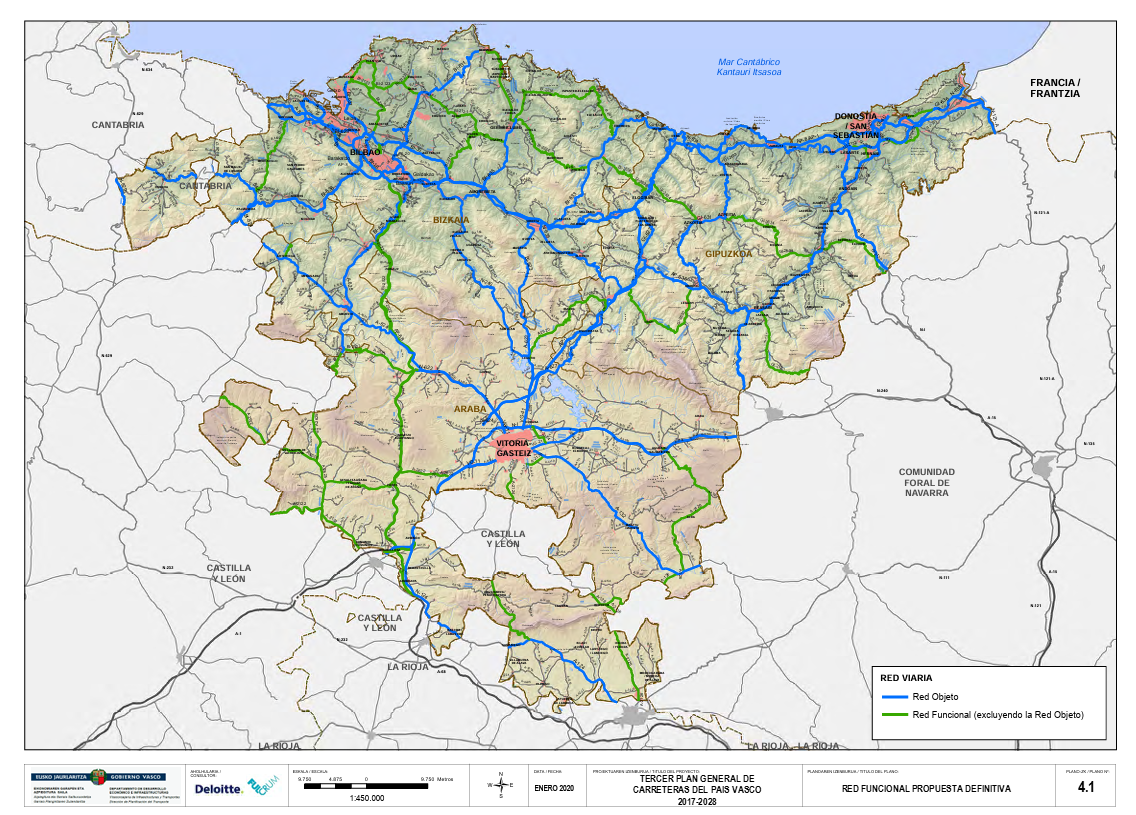
\includegraphics[scale=0.5]{includes/red_viaria_capv.png}
	\caption[Red viaria de la CAPV, extraído del Tercer Plan General de Carreteras del País Vasco 2017-2028. Fuente: https://www.euskadi.eus/tercer-plan-general-de-carreteras-del-pais-vasco-2017-2028/web01-a2bideko/es/]{Red viaria de la CAPV}
	\label{fig:red_viaria}
\end{figure}


En la figura \ref{fig:red_viaria} se aprecia la complejidad de la red viaria en la \acrshort{capv}. En diversas zonas como los accesos a Bilbao, los túneles del Kadagua o los enlaces con la A-8, se producen episodios de congestión recurrentes, especialmente en horas punta y durante condiciones meteorológicas adversas. Aunque Bizkaia dispone de una infraestructura \acrshort{its} notable (sensores, cámaras, estaciones meteorológicas), no se cuenta aún con herramientas predictivas suficientemente precisas que permitan anticipar estos episodios y facilitar la toma de decisiones en tiempo real.

La complejidad inherente a los datos de tráfico, caracterizados por correlaciones espacio-temporales, no linealidades y gran volumen, exige modelos capaces de capturar dichas relaciones con eficacia. Las aproximaciones tradicionales, basadas en regresión o aprendizaje automático clásico, resultan insuficientes en este contexto. Se necesita un enfoque moderno, capaz de integrar múltiples fuentes de datos y aprender representaciones complejas.

En respuesta a los retos mencionados, este trabajo propone el diseño, desarrollo y evaluación de un modelo de predicción del tráfico en Bizkaia basado en redes neuronales con arquitectura Transformer. Esta arquitectura ha demostrado un rendimiento sobresaliente en tareas de modelado secuencial y captura de dependencias a largo plazo, gracias a su mecanismo de atención, lo que la convierte en una candidata idónea para abordar la predicción de tráfico con alta precisión.

El modelo se alimentará de datos abiertos sobre tráfico y meteorología, publicados por organismos como Open Data Euskadi y Euskalmet, lo que garantiza la transparencia, replicabilidad y aplicabilidad del sistema propuesto. A través de un enfoque empírico, se evaluará la eficacia del modelo frente a enfoques tradicionales, utilizando métricas estándar y se estudiará su potencial para integrarse en sistemas actuales de gestión del tráfico.

Este documento se estructura de la siguiente manera: el capítulo 2 presenta una revisión del estado del arte, analizando los principales trabajos relacionados y su aplicabilidad al contexto de Bizkaia; el capítulo 3 define los objetivos del trabajo y la metodología seguida; los capítulos siguientes abordarán el desarrollo del proyecto y conclusiones finales, aunque esto es un trabajo por determinar.

\subsection{Introducción general del trabajo}

\vspace*{\fill}
\selectlanguage{spanish}
\begin{abstract}
	La predicción precisa del tráfico es clave para optimizar la movilidad y el uso de infraestructuras, especialmente en la \acrlong{capv} y más en concreto en la provincia de Bizkaia, donde la orografía, densidad urbana y condiciones meteorológicas suponen retos añadidos. Sin embargo, la complejidad inherente a los datos de tráfico, caracterizados por fuertes correlaciones espacio-temporales y patrones no lineales, dificulta su modelado y predicción exacta. Este trabajo propone un modelo de predicción basado en redes neuronales con arquitectura Transformer, capaz de capturar dependencias espacio-temporales complejas mediante mecanismos de atención que asignan pesos dinámicos a segmentos relevantes. Se emplearán datos abiertos de tráfico y meteorología procedentes de la provincia de Bizkaia. La validación se realizará con datos reales y se comparará frente a modelos tradicionales de redes neuronales, demostrando mejoras significativas en precisión. El sistema resultante ofrece una herramienta robusta y eficiente para la gestión del tráfico en tiempo real, con potencial para anticipar congestiones y optimizar la toma de decisiones operativas.
\end{abstract}
\textbf{Palabras clave}: Predicción del tráfico, Aprendizaje profundo, Transformers, Redes neuronales, Correlación espacio-temporal, Datos abiertos, Comunidad Autónoma del País Vasco, Bizkaia

\vfill

\selectlanguage{english}

\begin{abstract}
	Accurate traffic forecasting is essential for optimising mobility and infrastructure usage, especially in the Autonomous Community of the Basque Country (\acrshort{capv}) and particularly in the province of Bizkaia, where the region’s orography, urban density, and weather variability present additional challenges. However, the inherent complexity of traffic data, characterised by strong spatio-temporal correlations and non-linear patterns, makes its modelling and prediction difficult. This work proposes a prediction model based on neural networks with Transformer architecture, capable of capturing complex spatio-temporal dependencies through attention mechanisms that dynamically assign weights to relevant segments. Bizkaia's open traffic and weather datasets will be used. The model will be validated with real-world data and compared against traditional neural network models. The outcome will be a robust and efficient tool for real-time traffic management, with the potential to anticipate congestion and support the optimisation of operational decision-making.
\end{abstract}

\textbf{Keywords}: Traffic forecasting, Deep learning, Transformers, Neural networks, Spatio-temporal correlation, Open data, Autonomous Community of the Basque Country, Bizkaia
\selectlanguage{spanish}
\vspace*{\fill}
	\clearpage
	\section*{Contexto y estado del arte}
\label{sec:ctx_estart}
\addcontentsline{toc}{section}{Contexto y estado del arte}

En los últimos años, la predicción del tráfico se ha convertido en un campo de investigación clave dentro de los \acrlong{its}, impulsado por la disponibilidad creciente de datos en tiempo real y los avances en el aprendizaje automático. El objetivo principal es anticipar las condiciones del tráfico con suficiente precisión como para facilitar la toma de decisiones, tanto por parte de los operadores como de los usuarios de la red vial.

La problemática de la predicción del tráfico en entornos urbanos y regionales como Bizkaia presenta una elevada complejidad, debido a la naturaleza altamente dinámica y no lineal del flujo vehicular, así como por la influencia de factores exógenos como el clima, los eventos especiales o los accidentes. Esta complejidad ha motivado el desarrollo de una gran variedad de enfoques, desde modelos estadísticos clásicos hasta sofisticadas arquitecturas de aprendizaje profundo.

Este capítulo tiene como objetivo ofrecer un panorama de las principales técnicas, modelos y tecnologías utilizadas en la predicción del tráfico. A partir de una revisión sistemática de la literatura científica más relevante, se presentarán los enfoques predominantes y se analizará su aplicabilidad al caso concreto de Bizkaia. Finalmente, se establecerá un marco comparativo que servirá como punto de partida para justificar la solución propuesta en este trabajo.

\subsection{Técnicas existentes para la predicción del tráfico}

La literatura especializada distingue entre dos grandes familias de métodos para la predicción del tráfico: los modelos basados en estadística y los modelos basados en aprendizaje automático, con especial atención a los métodos de aprendizaje profundo. A continuación, se presenta una clasificación preliminar de las principales técnicas utilizadas:

\begin{itemize}
	\item \textbf{Modelos estadísticos}: \acrlong{arima}, Kalman Filter, regresiones lineales.
	\item \textbf{Modelos clásicos de machine learning}: \acrlong{svr}, \acrlong{rf}, \acrlong{knn}.
	\item \textbf{Redes neuronales profundas}:
	\begin{itemize}
		\item \acrlong{rnn}, \acrlong{lstm} y \acrlong{gru}.
		\item \acrlong{cnn}, para capturar relaciones espaciales.
		\item \acrlong{gnn}, incluyendo \acrlong{gcn} y \acrlong{gat}, adaptadas a redes viarias.
		\item Modelos Transformer.
	\end{itemize}
\end{itemize}

En las siguientes secciones, se revisarán con más detalle los fundamentos y aplicaciones de estas técnicas, poniendo el foco en los trabajos más relevantes que hayan utilizado estos enfoques en entornos comparables al del presente proyecto.

\subsubsection{Modelos estadísticos tradicionales}

Los modelos estadísticos tradicionales han sido fundamentales en la predicción del tráfico, especialmente en contextos donde se dispone de datos históricos limitados o se requiere una interpretación sencilla de los resultados. Estos modelos, incluyendo ARIMA, filtros de Kalman y regresiones lineales, permiten capturar patrones temporales y tendencias en los datos de tráfico, ofreciendo una base sólida para el desarrollo de sistemas de transporte inteligentes.

Los modelos \acrlong{arima} son herramientas estadísticas utilizadas para analizar y predecir series temporales. En el ámbito del tráfico, han demostrado ser eficaces para prever flujos vehiculares a corto plazo, especialmente en situaciones con patrones estacionales o tendencias lineales.

Por ejemplo, \cite{forecastArimaLtsm} aplicaron modelos \acrshort{arima} y \acrshort{lstm} para predecir el flujo de tráfico en la intersección de Muhima, Kigali, concluyendo que la combinación de ambos modelos mejora la precisión de las predicciones.

Asimismo, \cite{forecastSarima} propusieron un esquema de predicción utilizando el modelo \acrlong{sarima} para prever el flujo de tráfico a corto plazo con datos limitados, demostrando que es posible obtener predicciones precisas utilizando solo tres días de datos históricos.

El filtro de Kalman es un algoritmo recursivo que estima el estado de un sistema dinámico a partir de una serie de mediciones observadas, que contienen ruido y otras inexactitudes. En la predicción del tráfico, se utiliza para estimar y prever el flujo vehicular en tiempo real, adaptándose a cambios abruptos y condiciones variables.​

\cite{forecastKalman} emplearon el filtro de Kalman para predecir el flujo de tráfico a corto plazo en una carretera urbana de Dhaka, Bangladesh. El modelo logró un \acrlong{mape} del 14.62\%, indicando una precisión aceptable para aplicaciones prácticas.

La regresión lineal es una técnica estadística que modela la relación entre una variable dependiente y una o más variables independientes. En el contexto del tráfico, se ha utilizado para prever velocidades y flujos vehiculares basándose en variables como el tiempo, la densidad y la ocupación de la vía.​

Por ejemplo, \cite{liu2020congestion} desarrollaron un modelo de predicción del tiempo de congestión del tráfico utilizando análisis de regresión múltiple y análisis de supervivencia. El estudio demostró que el modelo de regresión lineal múltiple puede predecir con precisión el tiempo de congestión del tráfico, con un grado de ajuste entre el valor predicho y el valor real superior a 0.96. Este enfoque permitió identificar las características de distribución y duración de la congestión, proporcionando una base sólida para la predicción del tráfico en entornos urbanos.​

Sin embargo, estudios recientes han señalado limitaciones en la regresión lineal para capturar relaciones no lineales complejas en los datos de tráfico. Por ejemplo, en un análisis exhaustivo, se comparó el rendimiento de la regresión lineal con modelos más avanzados como \acrlong{rf} y XGBoost, encontrando que la regresión lineal presenta un ajuste deficiente y errores significativos en la predicción de velocidades de tráfico.

\subsubsection{Modelos clásicos de Machine Learning}

Los modelos clásicos de machine learning son métodos estadísticos avanzados capaces de abordar problemas complejos y no lineales. A continuación se describen brevemente tres técnicas destacadas: \acrlong{svr}, \acrlong{rf} y \acrlong{knn}, incluyendo ejemplos recientes de aplicaciones en la predicción del tráfico.

En cuanto a \acrfull{svr}, es una técnica basada en \acrfull{svm} que utiliza una función kernel para transformar el espacio de entrada original a uno de mayor dimensión, permitiendo modelar relaciones no lineales. El objetivo del \acrshort{svr} es identificar una función que tenga, como máximo, un error preestablecido (denominado \textit{margen}) respecto a los datos reales.

En el contexto de predicción de tráfico, \acrshort{svr} se ha mostrado eficaz debido a su robustez ante ruido y capacidad de generalización con muestras pequeñas. Por ejemplo, un estudio reciente aplicó \acrshort{svr} para predecir el volumen de tráfico a corto plazo utilizando datos de flujo vehicular recolectados en áreas urbanas, mostrando una precisión significativa en comparación con métodos \acrshort{lstm} de \cite{omar2024}.

\acrfull{rf} es un algoritmo basado en árboles de decisión, que genera múltiples árboles de forma independiente, utilizando subconjuntos aleatorios de datos de entrenamiento (bagging) y variables aleatorias. La predicción final se obtiene por consenso, promediando las predicciones individuales de cada árbol, lo que reduce considerablemente el riesgo de sobreajuste.

En el ámbito del tráfico, \acrshort{rf} es capaz de manejar grandes volúmenes de datos y capturar relaciones no lineales y complejas. Un ejemplo de aplicación es el estudio realizado por \cite{forecastRf}. El estudio tiene como objetivo predecir el flujo de tráfico a corto plazo, considerando patrones espaciales y temporales. Tras el preprocesamiento de datos con el Transformador Cuantil y la exploración de la correlación del flujo de tráfico, se identificaron los hiperparámetros óptimos del modelo mediante la búsqueda de cuadrícula de validación cruzada. El modelo \acrshort{rf} demostró el mejor rendimiento, alcanzando una alta precisión en la predicción del flujo de tráfico.

\acrfull{knn} es uno de los algoritmos más sencillos dentro de los métodos de aprendizaje supervisado. Este método predice el valor de una observación nueva en función de los valores de las K observaciones más cercanas del conjunto de entrenamiento. La cercanía se determina generalmente mediante una métrica de distancia, siendo la distancia euclidiana la más comúnmente utilizada.

A pesar de su simplicidad, \acrshort{knn} es muy eficaz en la predicción de tráfico cuando los patrones de flujo muestran alta dependencia espacial y temporal. Recientemente, \cite{forecastKnn} emplearon \acrshort{knn} para la predicción del tráfico en Bandung, Indonesia, empleando este método e integrado con la aplicación de simulación de movilidad urbana SUMO. El estudio buscó mitigar la congestión de tráfico anual en la ciudad, particularmente en periodos vacacionales. Utilizaron datos históricos de tráfico de Jl. Riau Bandung para predecir el nivel de congestión. La evaluación del rendimiento del método, usando una división de datos para entrenamiento y prueba, demostró una precisión muy alta con diferentes valores de 'k' vecinos considerados.

\subsubsection{Aprendizaje profundo}

El \textit{Deep Learning} o aprendizaje profundo es un área de \textit{Machine Learning} que utiliza redes neuronales artificiales de múltiples capas para modelar patrones complejos en los datos. Tras varias décadas de relativo estancamiento debido a las limitaciones computacionales y a las críticas vertidas por Minsky y Papert en los años 60 en el libro \textit{Perceptrons: An Introduction to Computational Geometry} \cite{minsky1969perceptrons}, las redes neuronales experimentaron un resurgimiento a partir de la década de los 2000, impulsado por el incremento exponencial de la capacidad de cómputo, la disponibilidad de grandes volúmenes de datos y el avance en algoritmos de entrenamiento. Este renacimiento del interés en las redes profundas se consolidó con el trabajo de \cite{hinton2006reducing}, donde se introdujo una técnica de preentrenamiento capa por capa utilizando autoencoders y máquinas de Boltzmann restringidas para facilitar el entrenamiento de redes neuronales profundas.

Sin embargo, fue en 2012 cuando el aprendizaje profundo irrumpió definitivamente en la comunidad científica, con la publicación de AlexNet, una red convolucional profunda que ganó con gran margen la competición ImageNet Large Scale Visual Recognition Challenge (ILSVRC). En este trabajo, Krizhevsky, Sutskever y Hinton demostraron que las redes profundas entrenadas con \acrlong{gpu} podían superar ampliamente los métodos tradicionales en tareas de visión por computador \cite{krizhevsky2012imagenet}. Este hito marcó el inicio de una nueva era para el aprendizaje profundo, consolidándolo como una de las herramientas más poderosas dentro del campo de la inteligencia artificial.

Actualmente, el aprendizaje profundo se caracteriza por la capacidad de representar funciones no lineales muy complejas gracias a estructuras como las redes neuronales profundas de tipo \acrlong{mlp}. Estas redes constan de múltiples capas ocultas, donde cada capa procesa información progresivamente más abstracta y permite descubrir patrones intrínsecos en grandes volúmenes de datos.

\subsubsection{Redes neuronales recurrentes}

Dentro del aprendizaje profundo, una clase especial de redes neuronales, conocidas como \acrfull{rnn}, ha demostrado ser particularmente efectiva para modelar secuencias temporales. Las \acrshort{rnn} están diseñadas para capturar dependencias temporales a largo plazo gracias a su estructura recurrente, que permite que la salida de una etapa de la red influya en etapas posteriores.

Las variantes más importantes y populares de las \acrshort{rnn} son las redes \acrlong{lstm} y \acrlong{gru}. Las \acrshort{lstm} fueron propuestas por \cite{hochreiter1997long}, y están especialmente diseñadas para manejar el problema del desvanecimiento del gradiente mediante el uso de puertas que controlan la información almacenada en la memoria de la red. Por otro lado, las redes \acrshort{gru}, introducidas por \cite{cho2014gru}, simplifican el modelo \acrshort{lstm} al combinar algunas de sus puertas, proporcionando un rendimiento similar con menos parámetros y una complejidad computacional reducida.

Diversos estudios han aplicado exitosamente las redes neuronales recurrentes a problemas específicos de predicción de tráfico, destacando las arquitecturas \acrshort{lstm} y \acrshort{gru}.

Un ejemplo notable es el trabajo realizado por \cite{zhao2017lstm}, en el que utilizaron una red neuronal \acrshort{lstm} para la predicción de flujo de tráfico a corto plazo. En su investigación, entrenaron un modelo con datos históricos de volumen vehicular recolectados en sensores, alcanzando un \acrfull{mre} de tan solo un 6,41\%, demostrando así la efectividad del enfoque \acrshort{lstm} para capturar patrones complejos en series temporales del tráfico.

En cuanto a la aplicación de redes \acrshort{gru}, cabe destacar el estudio llevado a cabo por \cite{ma2022cnn_gru}, quienes diseñaron un algoritmo híbrido basado en la combinación de \acrshort{cnn} y \acrshort{gru} para predecir la velocidad del tráfico. Este modelo obtuvo una media del \acrshort{mape} de aproximadamente 8,60\%, reflejando una considerable precisión en la predicción del flujo vehicular al integrar tanto características espaciales como temporales del tráfico.

Ambos estudios evidencian cómo el uso de redes neuronales recurrentes permite modelar con alta precisión las dependencias temporales complejas inherentes al tráfico vehicular, posicionándolas como una alternativa destacada frente a métodos clásicos o más tradicionales. Estos modelos son especialmente útiles en contextos de predicción a corto plazo, donde la precisión y la velocidad de respuesta son críticas para una gestión eficiente del tráfico y la toma de decisiones en tiempo real.

\begin{comment}
\subsubsection{Redes convolucionales}

Las \acrlong{cnn} son una clase de modelos de aprendizaje profundo diseñados para procesar datos con una estructura de tipo rejilla, como imágenes o series temporales espaciales. Su arquitectura se compone de capas convolucionales que aplican filtros para extraer características locales, seguidas de capas de agrupamiento y, finalmente, capas completamente conectadas para la toma de decisiones.​

En el contexto del tráfico vehicular, las \acrshort{cnn} son particularmente útiles para modelar la relación espacial entre diferentes segmentos de carretera y capturar patrones temporales en los datos de flujo de tráfico. Al representar los datos de tráfico en forma de matrices que reflejan la intensidad del tráfico en diferentes ubicaciones y momentos, las \acrshort{cnn} pueden aprender representaciones jerárquicas que facilitan la predicción precisa del flujo de tráfico.

La predicción precisa del flujo de tráfico es esencial para la gestión eficiente de las redes de transporte. Las \acrshort{cnn} permiten modelar las complejas interacciones espaciales y temporales presentes en los datos de tráfico, lo que resulta en predicciones más precisas y robustas. Además, su capacidad para manejar grandes volúmenes de datos y aprender características discriminativas las hace adecuadas para aplicaciones en tiempo real y sistemas de transporte inteligentes.

En el estudio \textit{WT-2DCNN: A convolutional neural network traffic flow prediction model} los autores \cite{forecastCnnWavelet} proponen un modelo que combina la transformada wavelet para la reconstrucción y descomposición de datos con una red neuronal convolucional bidimensional (2DCNN). Este enfoque permite manejar el ruido presente en los datos de tráfico y capturar características espaciales y temporales de manera más efectiva.​

La metodología aplicada consistía en los siguientes pasos. Para empezar, se aplica la transformada de wavelet para descomponer los datos de tráfico en componentes de diferentes frecuencias. Posteriormente, usa una 2DCNN para aprender las representaciones espaciales y temporales de los datos descompuestos y, para finalizar, se fusionan las características aprendidas para realizar la predicción del flujo del tráfico.

En consecuencia, el modelo WT-2DCNN demostró una mejora significativa en la precisión de la predicción del flujo de tráfico en comparación con métodos tradicionales, especialmente en escenarios con datos ruidosos.

En otro artículo científico titulado \textit{MF-CNN: Traffic Flow Prediction Using Convolutional Neural Network and Multi-Features Fusion}, los autores \cite{forecastMfCnn} presentan un modelo que integra múltiples características espaciales y temporales, así como factores externos como el clima y los días festivos, utilizando una red CNN para la predicción del flujo de tráfico.​

La metodología aplicada comienza por la extracción de características temporales a corto y largo plazo del flujo de tráfico. Seguidamente, se representan las características en matrices bidimensionales combinando dimensiones espaciales y temporales. A continuación, se aplica una \acrshort{cnn} para aprender las representaciones de las matrices y se finaliza fusionando las características aprendidas con factores externos mediante una capa de regresión logística para efectuar la predicción final.

Como resultado, el modelo MF-CNN logró una mejora notable en la precisión de la predicción del flujo de tráfico en comparación con varios modelos de referencia, demostrando la efectividad de integrar múltiples características y factores externos en el proceso de predicción.​
\end{comment}

\subsubsection{Graph Neural Networks}

Las \acrlong{gnn} surgen de la necesidad de extender las capacidades del aprendizaje profundo a datos no euclidianos, como los grafos, que representan relaciones complejas entre entidades. A diferencia de las redes neuronales tradicionales, que operan sobre datos estructurados en rejillas (como imágenes o secuencias), las \acrshort{gnn} están diseñadas para trabajar directamente con la estructura de los grafos, tal y como se explica por \cite{theoryGnn}, permitiendo capturar dependencias tanto locales como globales entre nodos.

Las GNN se basan en el principio de \textit{message passing}, donde cada nodo actualiza su representación en función de sus vecinos. Entre las arquitecturas más destacadas se encuentran:​

\begin{itemize}
	\item \textbf{\acrlong{gcn}}: Fueron introducidas en \cite{theoryGcn}. Estas redes generalizan las convoluciones a grafos, permitiendo una agregación eficiente de la información de los vecinos.
	\item \textbf{\acrlong{gat}}: Incorporan mecanismos de atención (como se verá más adelante) para ponderar la importancia de cada vecino en la actualización del nodo central. Fueron introducidas en \cite{theoryGan}.
	\item \textbf{\acrlong{ggnn}}: Utilizan mecanismos de puertas, similares a las \acrshort{lstm}, para controlar el flujo de información entre nodos.
\end{itemize}

La predicción del flujo de tráfico es un desafío clave en los sistemas de transporte inteligentes, donde es esencial anticipar las condiciones del tráfico para optimizar la movilidad urbana. Las \acrshort{gnn} son particularmente adecuadas para esta tarea debido a que las redes de carreteras pueden modelarse naturalmente como grafos, donde los nodos representan intersecciones o sensores, y las aristas representan las conexiones viales.

Un estudio destacado en este ámbito es \textit{Improving Traffic Density Forecasting in Intelligent Transportation Systems Using Gated Graph Neural Networks}, de \cite{forecastGgnn}. En este trabajo, los autores comparan diferentes arquitecturas de \cite{gnn} para la predicción de la densidad del tráfico, incluyendo \acrshort{gcn}, GraphSAGE y \acrshort{ggnn}. Los resultados muestran que las acrshort superan a las demás arquitecturas en términos de precisión, con un RMSE de 9.15 y un MAE de 7.1, destacando su capacidad para capturar dinámicamente las dependencias espaciales y temporales en los datos de tráfico.​

Otro estudio relevante es \textit{TrafficStream: A Streaming Traffic Flow Forecasting Framework Based on Graph Neural Networks and Continual Learning} de \cite{forecastGnn}. Este trabajo propone un marco de predicción de flujo de tráfico en tiempo real que combina \acrshort{gnn} con aprendizaje continuo, permitiendo adaptarse a cambios en la red de tráfico y patrones de flujo a lo largo del tiempo. El modelo utiliza estrategias como la reactivación de datos históricos y el suavizado de parámetros para mantener la precisión de las predicciones en entornos dinámicos.​

\subsubsection{Redes Neuronales con Transformers}

El avance hacia modelos más potentes y versátiles dentro del aprendizaje profundo encontró un punto de inflexión crucial en 2017 con la publicación del influyente artículo \textit{Attention is all you need} por \cite{attentionIsAllYouNeed}. Esta publicación revolucionó el campo del aprendizaje automático al introducir la arquitectura Transformer, una propuesta que eliminaba por completo el uso de estructuras recurrentes como \acrshort{rnn} o \acrshort{lstm}, en favor de un novedoso mecanismo de atención que permitía modelar relaciones de largo alcance en las secuencias de entrada, mediante el cómputo paralelo.

La clave de los Transformers reside en el \textbf{multi-head self-attention}, que otorga al modelo la capacidad de ponderar dinámicamente la importancia relativa de distintos elementos dentro de una secuencia. Este mecanismo, además de ofrecer un rendimiento computacional más eficiente, mejora la capacidad de aprendizaje del modelo frente a secuencias largas o ruidosas, lo que resulta particularmente útil en dominios complejos como la predicción del flujo del tráfico urbano.

A diferencia de las \acrshort{rnn}, que deben procesar las secuencias de manera secuencial, los Transformers permiten el aprendizaje paralelo y la captura simultánea de dependencias tanto locales como globales, lo que ha demostrado ser especialmente relevante para modelar patrones espacio-temporales complejos.

\vspace{0.5cm}

El uso de modelos Transformer en el ámbito de los sistemas inteligentes de transporte ha crecido significativamente en los últimos años, debido a su capacidad para capturar interacciones complejas entre nodos de una red vial y su evolución en el tiempo.

Un estudio reciente y particularmente relevante para este trabajo es el desarrollado por \cite{trafficformer}, titulado \textit{Transformer-based short-term traffic forecasting model considering traffic spatiotemporal correlation}. En este artículo, los autores presentan \textbf{Trafficformer}, un modelo Transformer adaptado específicamente a la predicción del tráfico a corto plazo, integrando correlaciones espacio-temporales mediante máscaras espaciales y representaciones topológicas de la red viaria.

En cuanto a la arquitectura, el modelo Trafficformer consta de tres módulos fundamentales: 
\begin{itemize}
	\item[(1)] Extracción de características temporales mediante \acrlong{mlp}. 
	\item[(2)] Interacción espacial basada en codificadores Transformer con máscaras de atención topológicas. 
	\item[(3)] Predicción de velocidades mediante una red \acrshort{mlp} final. 
\end{itemize}

Esta arquitectura fue evaluada con el conjunto de datos del \textit{Seattle Loop Detector Dataset}, superando a modelos clásicos como ARIMA, \acrshort{svr} y también a redes profundas como \acrshort{lstm}+\acrshort{mlp} y TGG-LSTM, tanto en precisión (\acrshort{mae}, \acrshort{mape}, \acrshort{rmse}) como en eficiencia computacional.

La inclusión de una máscara espacial, que filtra interacciones irrelevantes basándose en la topología vial y el tiempo de viaje entre nodos, permitió al modelo enfocarse en relaciones espacialmente significativas, lo que se tradujo en una mejora del 18\% en precisión frente a modelos equivalentes sin esta optimización. Esta capacidad de interpretar relaciones espaciales relevantes es fundamental en contextos como el tráfico urbano, donde las dependencias no son uniformes ni euclidianas, y dependen del trazado real de la red viaria.

\vspace{0.5cm}

El trabajo de \cite{trafficformer} demuestra que los modelos basados en Transformers no sólo son competitivos, sino que se posicionan como una opción de referencia para tareas de predicción del tráfico, permitiendo una mejor generalización, mayor interpretabilidad y adaptabilidad frente a cambios dinámicos en la red.

Este enfoque supone un salto cualitativo respecto a técnicas previas como \acrshort{lstm}, \acrshort{gru} o incluso \acrshort{gnn}, al combinar lo mejor de los modelos de secuencia (captura temporal) con mecanismos estructurados de atención espacial. Además, su arquitectura modular y altamente paralelizable lo convierte en un candidato ideal para despliegues en entornos cloud, edge o híbridos, como los requeridos en la infraestructura del proyecto que nos ocupa.

Por todo ello, este modelo ha sido seleccionado como piedra angular sobre la cual se desarrollará la propuesta metodológica del presente trabajo, tanto en la fase de experimentación como en el diseño arquitectónico del modelo final.

\subsection{Ventajas del uso de Transformers frente a otras arquitecturas}

La arquitectura Transformer representa un avance significativo respecto a los modelos secuenciales (\acrshort{lstm} o \acrshort{gru}) y estructurales (como las \acrshort{gnn}), tanto desde el punto de vista teórico como práctico.

En primer lugar, los modelos secuenciales dependen fuertemente del procesamiento secuencial, lo que limita la paralelización durante el entrenamiento y puede llevar a problemas de desvanecimiento o explosión del gradiente (leer en \cite{desvGradiente}) en secuencias largas. Aunque han demostrado buen rendimiento en predicción temporal, su capacidad para modelar relaciones espaciales complejas es limitada. Por otro lado, las \acrshort{gnn} destacan en la modelización espacial, pero presentan dificultades cuando se requiere combinar relaciones topológicas con dinámicas temporales de forma eficaz.

Los Transformers, y en particular la arquitectura Trafficformer, superan estas limitaciones al:

\begin{itemize}
	\item \textbf{Separar explícitamente los componentes espaciales y temporales}: Trafficformer utiliza una \acrshort{mlp} para extracción temporal y un codificador Transformer para interacción espacial, optimizando cada fase por separado.
	\item \textbf{Utilizar multi-head self-attention con enmascaramiento espacial}: Esto permite al modelo centrarse solo en las interacciones viales relevantes, mejorando la eficiencia y la precisión.
	\item \textbf{Permitir entrenamiento completamente paralelo}: Gracias al mecanismo de atención, el modelo puede ser entrenado de manera más rápida que una \acrshort{rnn} convencional.
\end{itemize}

Los resultados experimentales de \cite{trafficformer} muestran que Trafficformer supera consistentemente a las otras propuestas mencionadas anteriormente en múltiples métricas de evaluación como \acrshort{mae}, \acrshort{rmse} y \acrshort{mape}. Por ejemplo, en el dataset del \textit{Seattle Loop Detector}, se observó una mejora de hasta el 18\% en error medio absoluto frente a los mejores modelos recurrentes. Además, la arquitectura Transformer mostró una mayor capacidad de generalización frente a cambios dinámicos del tráfico. En la tabla \ref{tab:comparativa_modelos} se puede ver a modo resumido todo lo dicho anteriormente.

\begin{table}[H]
	\centering
	\caption{Comparativa entre arquitecturas en tareas de predicción del tráfico}
	\label{tab:comparativa_modelos}
	\renewcommand{\arraystretch}{1.4}
	\begin{tabularx}{\textwidth}{lXXX}
		\toprule
		\textbf{Aspecto} & \textbf{RNNs (LSTM, GRU)} & \textbf{GNNs} & \textbf{Transformers} \\
		\midrule
		Procesamiento secuencial vs. paralelo &
		Procesamiento secuencial con paralelización limitada &
		No aplicable (estructura estática) &
		Paralelización total mediante mecanismo de atención \\
		
		\midrule
		Modelado espacial y temporal &
		Modelado temporal fuerte, pero poco eficiente para relaciones espaciales &
		Excelente modelado espacial, dificultad para integrar dinámica temporal &
		Modelado explícito y desacoplado de componentes espaciales y temporales \\
		
		\midrule
		Rendimiento empírico &
		Rendimiento limitado en benchmarks de tráfico &
		Rendimiento moderado en tareas espaciales, sensible a ruido temporal &
		Mejores resultados en métricas MAE, RMSE y MAPE, mayor capacidad de generalización \\
		\bottomrule
	\end{tabularx}
\end{table}

En resumen, los modelos Transformer no solo ofrecen ventajas computacionales, sino que proporcionan una representación más rica y eficiente de las correlaciones espacio-temporales que caracterizan al problema de la predicción del tráfico urbano. 
	\clearpage
	\section*{Objetivos y metodología de trabajo}
\label{sec:obj_metd}
\addcontentsline{toc}{section}{Objetivos y metodología de trabajo}

En este capítulo se exponen los objetivos perseguidos con el desarrollo del presente Trabajo Fin de Máster, pasando por la infraestructura y tecnologías seleccionadas, y acabando con la metodología empleada para su ejecución. El trabajo se enmarca dentro del área del aprendizaje profundo, aplicados al problema de la predicción del flujo de tráfico urbano. El propósito es diseñar una solución capaz de anticipar el estado de la red viaria a corto plazo en la provincia de Bizkaia, utilizando datos abiertos y públicos de fuentes institucionales, lo cual permitirá evaluar tanto la capacidad de generalización de los modelos como su utilidad práctica en un contexto real. 

Como se analizó en el capítulo anterior, la predicción del tráfico urbano enfrenta importantes retos derivados de la alta variabilidad temporal y la compleja dependencia espacial de los datos. Entre los trabajos analizados, destaca el modelo Trafficformer de \cite{trafficformer}, que introduce un enfoque basado en Transformers mejorado mediante máscaras espaciales para filtrar ruido y enfocar la atención en interacciones relevantes entre nodos de la red. Aunque el modelo original fue diseñado para predecir velocidades de tráfico, su arquitectura resulta igualmente aplicable a la predicción de volúmenes de tráfico, esto es, la cantidad de vehículos que circulan por un punto dado en cada intervalo temporal, mediante una adaptación del preprocesamiento y del objetivo del modelo.

\subsection{Objetivos del proyecto}

El objetivo general de este Trabajo Fin de Máster es el diseño, implementación y evaluación de un sistema de predicción del tráfico urbano a corto plazo mediante el uso de técnicas de aprendizaje profundo, con especial énfasis en las redes neuronales de tipo Transformer. La solución desarrollada debe ser capaz de predecir con precisión el estado futuro del tráfico en diversos puntos de la red viaria de Bizkaia, aprovechando el valor añadido que ofrecen los datos abiertos procedentes de fuentes públicas, como los portales de Open Data del Gobierno Vasco. Para ello, se debe implementar y entrenar un modelo de predicción inspirado en el modelo Trafficformer, adaptado a volúmenes de tráfico. Este objetivo principal responde a la necesidad creciente de disponer de herramientas tecnológicas que permitan mejorar la gestión de la movilidad en entornos urbanos, facilitar la toma de decisiones estratégicas y operativas en tiempo real, y anticiparse a situaciones potenciales de congestión. La precisión de la predicción se configura como un factor clave en la eficacia de sistemas \acrshort{its} modernos, especialmente en contextos densamente poblados como el área metropolitana de Bilbao. 

Como primer objetivo específico se pretende analizar el conjunto de datos disponibles en el catálogo de datos abiertos del Gobierno Vasco ubicado en \cite{openDataGv}. Dentro del mismo, se pretende identificar y analizar el Api de tráfico de \cite{apiTraffic}, además de otros factores contextuales como la meteorología, que se ha demostrado influyente en la dinámica del tráfico y cuyo \acrshort{api} se ubica en \cite{apiMeteo}.

Asimismo, se plantea como segundo objetivo específico la validación empírica de los modelos mediante experimentación con datos reales, evaluando su rendimiento con métricas reconocidas en el ámbito de la predicción, tales como el error cuadrático medio o \acrshort{rmse}, el error absoluto medio o \acrshort{mae} o el error porcentual absoluto medio o \acrshort{mape}. La comparación entre distintos enfoques permitirá identificar las ventajas y limitaciones de cada uno, así como proponer mejoras que potencien su aplicabilidad.

Por último, se considera el tercer objetivo específico del trabajo ofrecer una reflexión crítica sobre el impacto potencial de este tipo de soluciones en el ámbito de la movilidad urbana y su eventual integración en sistemas de ayuda a la decisión de carácter público o privado. El valor añadido que se pretende aportar no reside únicamente en la capacidad predictiva del modelo, sino también en su posible contribución al desarrollo de una movilidad más eficiente, sostenible e inteligente.

\subsection{Infraestructura y tecnologías empleadas}

En este apartado se van a exponer todos los recursos seleccionados que van a servir de soporte para la consecución de los objetivos y el desarrollo del proyecto.

Para ello, se va a utilizar una infraestructura híbrida compuesta por recursos locales y servicios en la nube.
Como equipo de desarrollo se va a seleccionar el equipo personal, que se compone por un procesador Intel Core i7-10700K de 10ª generación desbloqueado, con 32 GB de memoria \acrshort{ram} DDR4, haciendo uso de 2 discos \acrshort{ssd} NVMe (512 GB + 1 TB) y un HDD de 2 TB como almacenamiento, equipado con una GPU Nvidia GTX 1070 con soporte CUDA y corriendo el Sistema Operativo Windows 11 Pro.

Este equipo permitirá realizar tareas de programación, experimentación y entrenamiento preliminar, si bien se anticipa que no será suficiente para entrenar modelos de gran tamaño o con grandes cantidades de datos.

Por ello, se deberá emplear una infraestructura remota para realizar los distintos entrenamientos. Dada la necesidad de cómputo intensivo, se contempla el uso de una instancia EC2 en Amazon Web Services (AWS), con una AMI optimizada para entrenamiento de modelos con PyTorch (por ejemplo, la AMI de Deep Learning de AWS con soporte GPU Tesla T4 o V100). Esta infraestructura permitirá acelerar significativamente el proceso de entrenamiento y validación.

Asimismo, se va a hacer uso de un servidor doméstico con \href{https://www.truenas.com/}{TrueNAS} Scale Electric Eel como sistema operativo, equipado con un procesador Intel Core i5-7400 de 7ª generación, con 16 GB de RAM DDR4 y dos discos duros de 4 TB configurados en RAID 1. Este servidor albergará una base de datos \href{https://www.mongodb.com/}{MongoDB} para almacenamiento estructurado de datos y \href{https://min.io/}{MinIO} como sistema de almacenamiento tipo S3, útil para almacenamiento masivo y backups. Todos esos servicios van a funcionar como contenedores \href{https://www.docker.com/}{Docker}.

En cuanto al software, se van a seleccionar los lenguajes de programación \href{https://kotlinlang.org/}{Kotlin} (con \href{https://gradle.org/}{Gradle} como herramienta de construcción) y \href{https://www.python.org/}{Python} (con \href{https://python-poetry.org/}{Poetry} como gestor de dependencias y de empaquetamiento). En cuanto a los entornos de desarrollo, se ha decidido hacer uso de la suite de Jetbrains, puesto que facilitan licencias para estudiantes y son muy completas (ofreciendo muchas funcionalidades y asistentes que hacen más productiva tu jornada). Estos IDE son \href{https://www.jetbrains.com/es-es/idea/}{IntelliJ IDEA} (para el desarrollo con Kotlin) y \href{https://www.jetbrains.com/es-es/pycharm/}{PyCharm} (para el desarrollo con Python). Para el control de versiones se va a emplear \href{https://git-scm.com/}{Git}, con repositorios en GitHub o GitLab.

Para el desarrollo del modelo de predicción de tráfico se ha optado por utilizar \href{https://pytorch.org/}{PyTorch} como backend principal. Esta decisión se fundamenta en la flexibilidad que ofrece esta biblioteca para la implementación de arquitecturas avanzadas, como redes neuronales recurrentes (LSTM, GRU), redes convolucionales (CNN), Graph Attention Networks (GAT) y modelos basados en Transformers. Además, PyTorch cuenta con una comunidad investigadora muy activa y un ecosistema maduro que incluye librerías especializadas como PyTorch Geometric o HuggingFace Transformers, altamente relevantes para el ámbito de este trabajo. A diferencia de otros entornos como TensorFlow/Keras, que destacan por su facilidad de uso en fases de prototipado, PyTorch ofrece un control más explícito sobre el flujo de datos y la personalización del entrenamiento, lo que resulta especialmente valioso en proyectos que requieren ajustar arquitecturas de manera específica para capturar correlaciones espaciotemporales complejas en el tráfico urbano. 

Estas decisiones se ven respaldadas por análisis comparativos recientes, como el realizado por DataCamp, donde se destaca que \textit{PyTorch} suele ser más rápido y proporciona mejores capacidades de depuración que \textit{Keras}. Estas características lo hacen especialmente adecuado para entornos de investigación y desarrollo de modelos complejos cite{datacamp2023}.

Además, UnfoldAI ofrece un análisis detallado sobre las fortalezas y debilidades de los principales frameworks de aprendizaje profundo. En su estudio comparativo se destaca que \textit{PyTorch} proporciona una mayor flexibilidad y control, lo que lo convierte en la opción preferida en entornos de investigación, mientras que \textit{Keras} sobresale por su simplicidad y facilidad de uso, resultando ideal para usuarios principiantes y tareas de prototipado rápido \cite{unfoldai2024}.

\subsection{Metodología de trabajo}

Para la consecución de los objetivos, tomando como referencia la solución Trafficformer, se ha pensado en estructurar el proyecto de la siguiente manera:

\begin{itemize}
	\item Adquisición y preprocesamiento de datos.
	\begin{itemize}
		\item \textbf{Datos}: se utilizarán datos abiertos provenientes del portal Open Data de Euskadi, principalmente de sensores que registran el número de vehículos que atraviesan puntos específicos de la red viaria en intervalos regulares.
		\item \textbf{Preprocesamiento}: se realizará la agregación temporal si es necesario (por ejemplo, a intervalos de 5 minutos), imputación de valores perdidos, normalización y generación de ventanas deslizantes para construir las series históricas.
	\end{itemize}
	\item Arquitectura del modelo. La arquitectura seguirá los principios del modelo Trafficformer, la cual se puede apreciar en la figura \ref{fig:trafficformer}, con los siguientes componentes adaptados:
	\begin{itemize}
		\item \textbf{Extracción temporal}: un MLP de dos capas se encargará de extraer patrones no lineales de las series de volumen de vehículos por punto de control.
		\item \textbf{Máscara espacial}: se construirá una matriz de adyacencia basada en la topología de la red viaria, utilizando distancias reales o tiempos de viaje para definir relaciones de vecindad relevantes.
		\item \textbf{Codificador Transformer}: mediante multi-head attention, el modelo extrae relaciones espaciales entre nodos cercanos, permitiendo una representación contextualizada del tráfico.
		\item \textbf{Predicción}: se proyectan las representaciones espacio-temporales a una predicción del número de vehículos que circularán por cada punto de la red en el siguiente intervalo.
	\end{itemize}
	\item Entrenamiento y evaluación.
	\begin{itemize}
		\item \textbf{Métricas}: se utilizarán MAE, RMSE y MAPE para comparar la predicción de conteos de vehículos.
		\item \textbf{Modelos base}: se tendrá como referencia el modelo \acrshort{mlp} desarrollado anteriormente.
		\item \textbf{Validación}: se aplicará validación temporal (walk-forward) para simular condiciones reales de predicción.
	\end{itemize}
\end{itemize}

\begin{figure}[H]
	\centering
	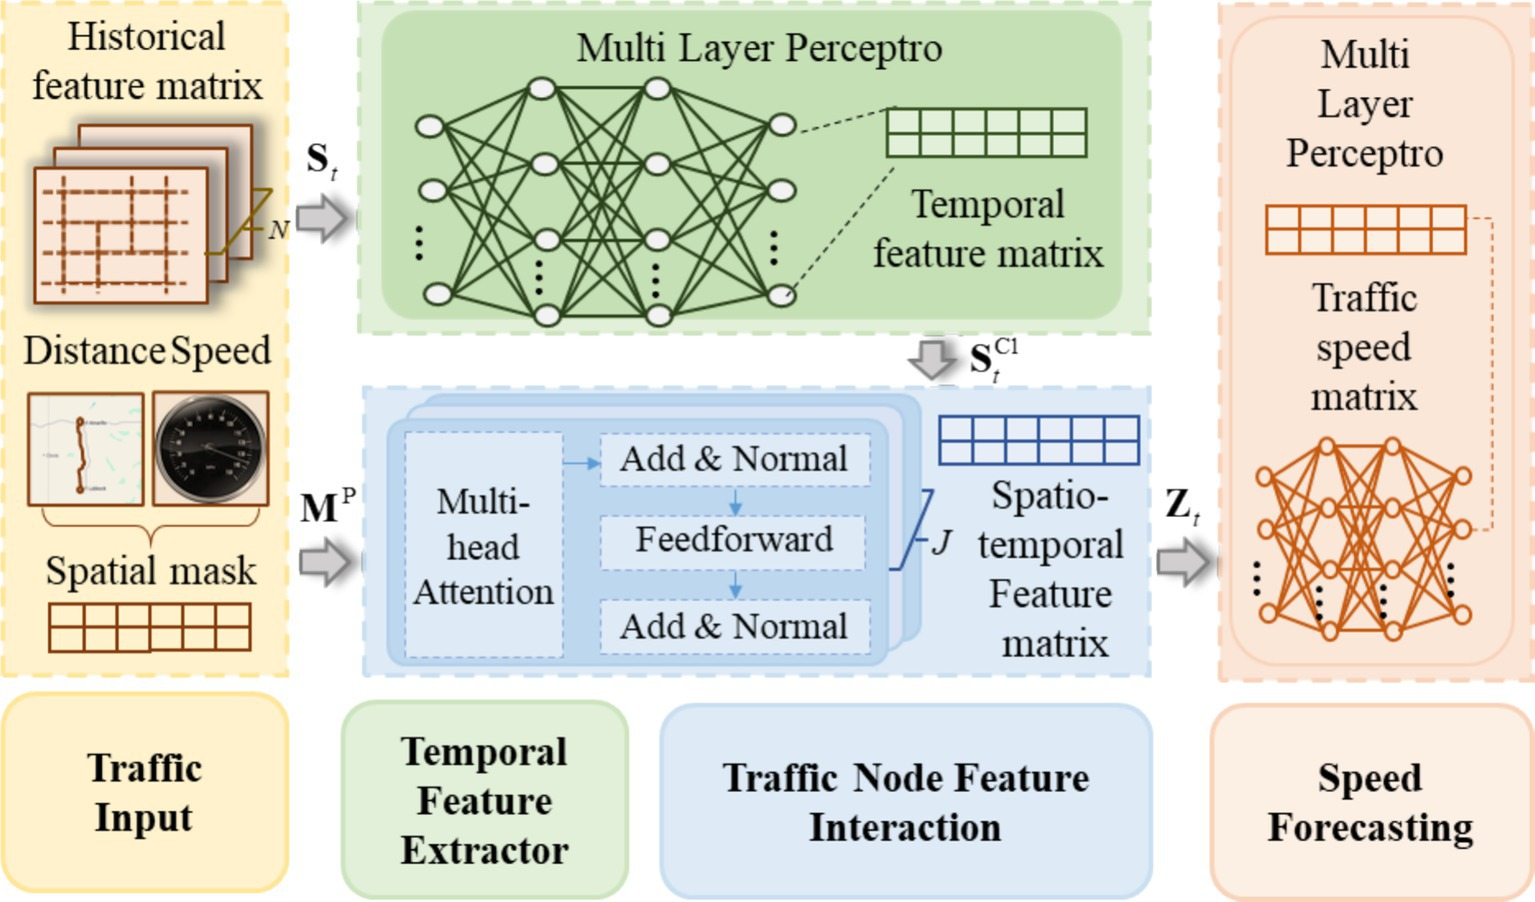
\includegraphics[width=0.9\textwidth]{includes/fnbot-19-1527908-g001.jpg}
	\caption{Arquitectura general del modelo Trafficformer \cite{trafficformer}}
	\label{fig:trafficformer}
\end{figure}

Como consecuencia, se prevé llevar a cabo las siguientes tareas.

\begin{itemize}
	\item Extracción y almacenamiento de datos. Desarrollo de un módulo en Kotlin para conectar con las \acrshort{api} públicas de tráfico y meteorología de Open Data Euskadi. Almacenamiento de los datos crudos en MongoDB y objetos binarios (imágenes, CSVs temporales) en MinIO.
	\item Preprocesamiento y transformación de datos. Conversión de datos crudos en estructuras listas para entrenamiento, mediante scripts en Python. Aplicación de técnicas de normalización, resampleo temporal y gestión de datos faltantes.
	\item Entrenamiento de modelos neuronales. Implementación de un modelo base \acrshort{mlp} para establecer una línea base de rendimiento. Posterior implementación de un modelo Transformer adaptado al tráfico, con atención espacio-temporal y uso de máscaras de conectividad vial.
	\item Evaluación comparativa. Evaluación de los modelos con un conjunto de métricas estándar (\acrshort{mae}, \acrshort{rmse}, \acrshort{mape}). Comparativa entre modelos para seleccionar el más adecuado para el caso de uso.
	\item Validación y conclusiones. Validación en escenarios reales y extracción de conclusiones sobre la utilidad del modelo. Estudio de la viabilidad de su aplicación en entornos reales, como el soporte a \acrshort{its} o planificación urbana.
\end{itemize}

	\clearpage
	
	%\section{Introducción}
\iffalse
Ejemplo enumeración:
\begin{enumerate}
	\item Item1
	\item Item2
\end{enumerate}
Aquí se referencia a la imagen \ref{prueba} y aquí a la imagen \ref{prueba_invertida}

Ejemplo figura:
\begin{figure}[h]
	\centering
	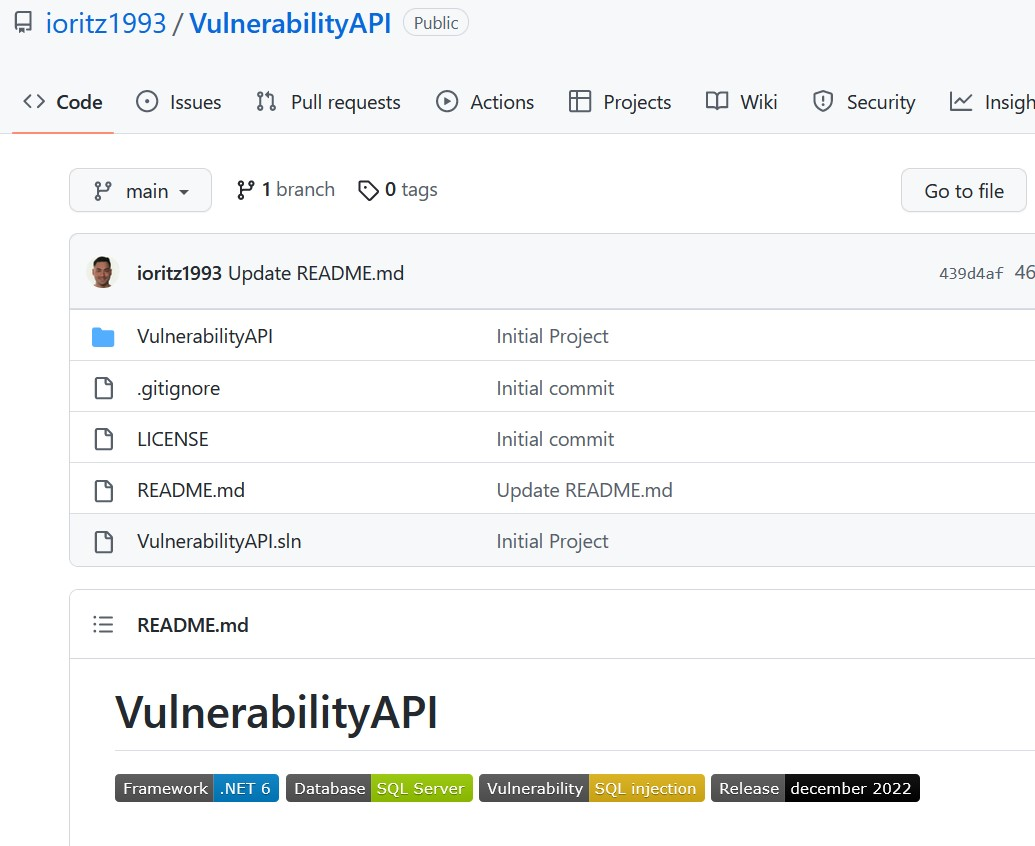
\includegraphics[width=160mm]{includes/ejemplo_figura.jpg}
	\caption[Ejemplo figura]{Ejemplo figura (Elaboración propia)}
	\label{prueba}
\end{figure} 

\begin{figure}[h]
	\centering
	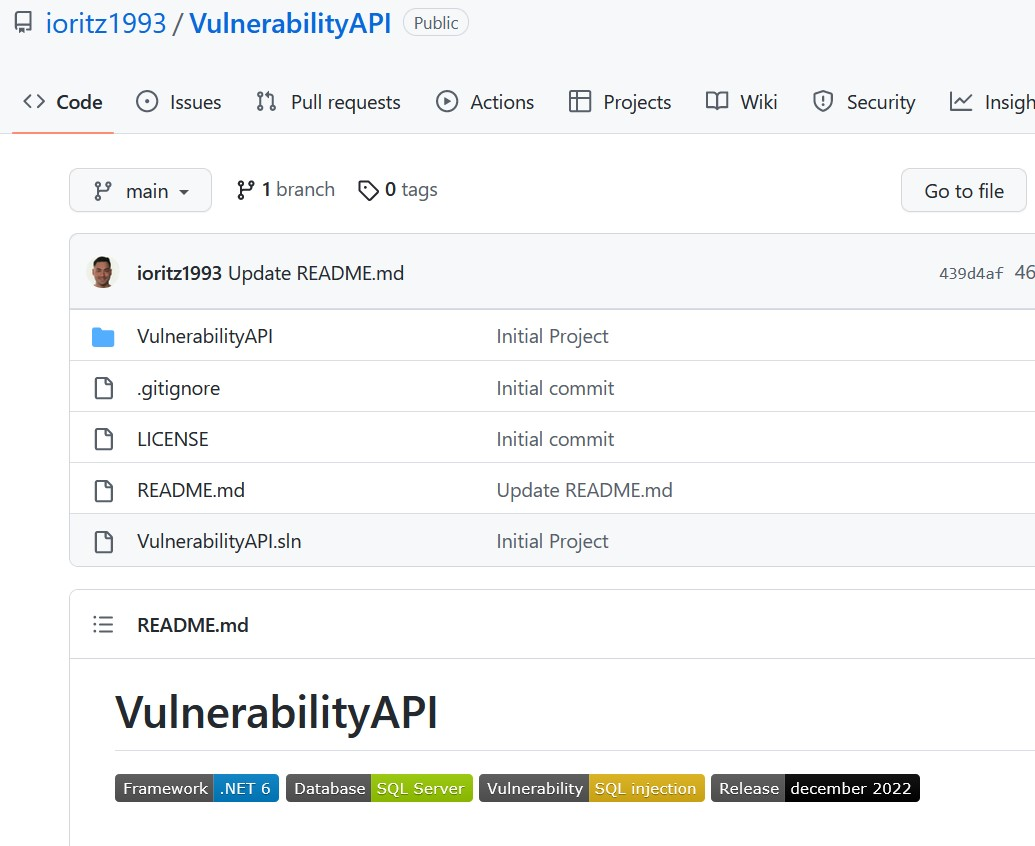
\includegraphics[width=160mm, angle=180]{includes/ejemplo_figura.jpg}
	\caption[Ejemplo figura girada]{Ejemplo figura girada (Elaboración propia)}
	\label{prueba_invertida}
\end{figure} 
\fi

La movilidad urbana eficiente se ha convertido en un reto prioritario para las administraciones públicas, especialmente en territorios con alta densidad poblacional y complejidad geográfica. La creciente demanda de desplazamientos, junto con la necesidad de garantizar la sostenibilidad del sistema de transporte, exige soluciones avanzadas que permitan optimizar el uso de las infraestructuras existentes y reducir los impactos negativos del tráfico. Una gestión adecuada del tráfico no solo repercute en la calidad de vida de la ciudadanía, sino que también incide directamente en la reducción del consumo energético, la mejora de la seguridad vial y la disminución de la contaminación atmosférica.

En la provincia de Bizkaia, estos desafíos se intensifican debido a varios factores estructurales y ambientales. Por un lado, su orografía accidentada limita la expansión de la red vial y concentra los flujos de tráfico en determinados corredores estratégicos. Por otro, la alta concentración urbana en el área metropolitana de Bilbao genera elevados niveles de congestión, especialmente en horas punta. Además, la variabilidad meteorológica, con episodios frecuentes de lluvia o niebla, puede alterar de forma significativa las condiciones de circulación, introduciendo incertidumbre en la gestión diaria del tráfico.

En este contexto, la predicción del tráfico emerge como una solución clave, al permitir estimar de forma anticipada el comportamiento del flujo vehicular a partir del análisis de datos históricos y condiciones externas. Durante los últimos años, el avance en el ámbito de la inteligencia artificial, y en particular del aprendizaje profundo, ha facilitado la creación de modelos cada vez más precisos para esta tarea. Entre las arquitecturas más prometedoras se encuentra la basada en Transformers, ampliamente reconocida por su capacidad para modelar dependencias a largo plazo y procesar grandes volúmenes de datos secuenciales con eficiencia.

Este trabajo tiene como objetivo el desarrollo de un modelo predictivo basado en Transformers, enfocado específicamente en el entorno de Bizkaia, y alimentado con datos abiertos de tráfico y meteorología publicados por organismos públicos. Se busca con ello generar una solución tecnológica que permita anticipar de manera fiable el estado del tráfico en distintas zonas del territorio y contribuir así a una gestión más inteligente, preventiva y sostenible de la movilidad urbana.

El trabajo se va a estructurar de la siguiente forma. Para comenzar, se va a contextualizar el problema y se van a definir los objetivos, detallando los retos del tráfico en Bizkaia y justificando la necesidad del modelo previsto. Posteriormente, se va a definir la metodología que se va a seguir. Seguidamente, se va a realizar el estudio del estado del arte, recogiendo las principales aproximaciones en cuanto a técnicas para la predicción del tráfico. A continuación, se abordará el desarrollo específico del modelo propuesto, incluyendo todas las fases implicadas en su diseño, entrenamiento y validación. Para finalizar, se presentarán distintas opciones en cuanto a trabajo futuro a llevar a cabo y se expondrán las conclusiones extraídas.


	%\clearpage
	%\section{Justificación}
\iffalse
 Ejemplo referencia \citep{ejemploReferencia}.\par
 Ejemplo acrónimo \gls{sdr}\\
 Ejemplo segunda llamada a acrónimo \gls{sdr}
 Ejemplo tabla \ref{ejemploTabla}
 
 
 \begin{table}[h]
 	\centering
 	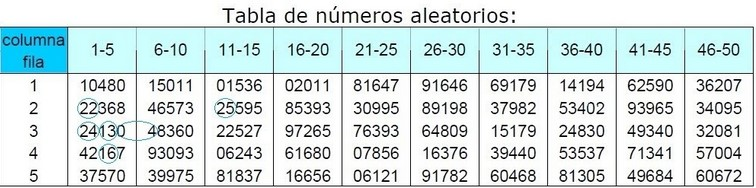
\includegraphics[width=100mm]{includes/ejemplo_tabla.jpg}
 	\caption[Tabla números aleatorios]{Tabla números aleatorios \citep{ejemploReferencia}}
 	\label{ejemploTabla}
 \end{table}
 Como en el caso anterior, la tabla \ref{cochesAfectados} sólo muestra un pequeño porcentaje de coches afectados.
\fi


	%\clearpage
	%\section{Section}
\lipsum[1-1]
\subsection{Subsection}
\lipsum[1-1]

	%\clearpage
	%\section{Section}
\lipsum[1-1]
\subsection{Subsection}
\lipsum[1-1]
\subsubsection{Subsubsection}
\lipsum[1-1]
\paragraph{Paragraph}
\lipsum[1-1]
\subparagraph{Subparagraph}
\lipsum[1-1]
	%\clearpage
	%\section{Section}

	%\clearpage
	%\section{Section}
\lipsum[1-1]

	%\clearpage
	%\section{Trabajos futuros}
\lipsum[1-1]
	%\clearpage
	%\section{Conclusiones}
\lipsum[1-1]

	\clearpage
	\printglossary[type=\acronymtype,title={Lista de Acrónimos y Abreviaturas}]
	\glsaddallunused

	\clearpage
	\phantomsection %Insertamos ancla en la bibliografía para hipervínculo
	\begin{flushleft}
		%Visualizar bibliografía con notice incluida la no citada
		\nocite{*}
		\bibliographystyle{apacite}
		\bibliography{recursos/bibliografia}
	\end{flushleft}

% Cuando tengamos apéndices, mostrar aquí
%	\clearpage
%	\appendix
%	\section{Código de la solución}

\lipsum[1-1]
\end{document} 